
\section{Search friendliness}

Of course, the most important usability concern for a course explorer/scheduler is being able to effectively \emph{find courses}.

In this section, I will present the \emph{Skedge DSQL}, a domain-specific query language that is based on natural language. Next, I will demonstrate how Skedge leverages the DSQL to handle the three search criteria students have for finding courses better than CDCS does.

\subsection{Natural language search}

In the spirit of this chapter's theme, Skedge's search method was, again, primarily designed as a reaction to CDCS's. CDCS's search method is a 15-field form (see Figure \ref{fig:cdcs-search}), of which I only found myself regularly using two (one of them being the \emph{required} ``Year/Term'' field). This prompted me to closely examine the fields to a) determine redundancies between them and b) find how to make some of the valuable filter fields more usable. From this came Skedge's unified, natural language based search method, which I call the \emph{Skedge Domain-Specific Query Language (Skedge DSQL)}. Figure \ref{fig:sk-search} is a list of example possible searches shown to users as they type.

\begin{figure}[ht]
  \centering
  \vspace{5pt}
  \begin{tabular}{c c}
    \begin{subfigure}[w]{4.5cm}
      \centering
      \fbox{
        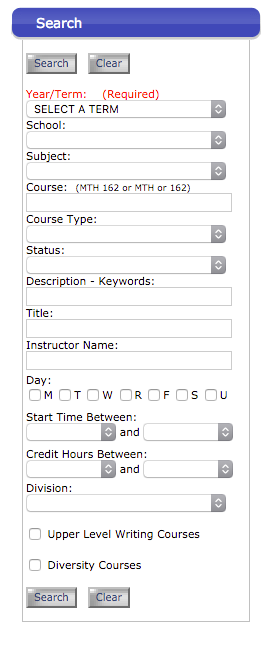
\includegraphics[width=3.3cm]{images/cdcs/search}
      }
      \caption{Form-based search in CDCS} \label{fig:cdcs-search}
    \end{subfigure}
    \hspace{5pt}
    \begin{subfigure}[w]{8.5cm}
      \centering
      \fbox{
        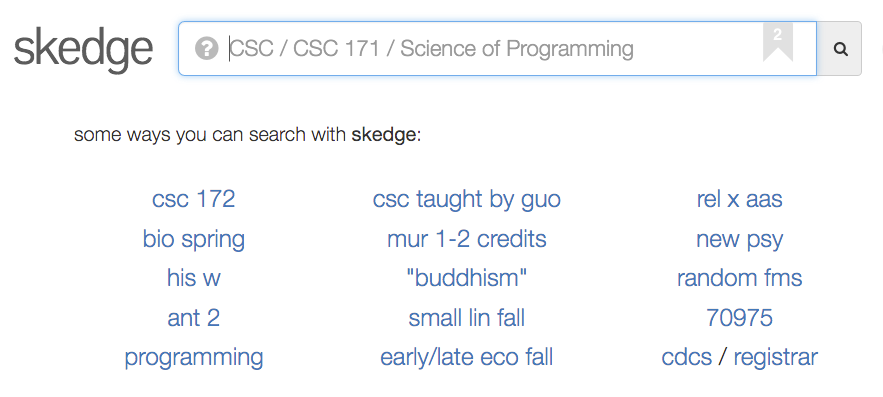
\includegraphics[width=1.00\textwidth]{images/skedge/search}
      }
      \caption{Examples of the Skedge DSQL} \label{fig:sk-search}
    \end{subfigure}
  \end{tabular}
  \caption{Two philosophies of search method}
\end{figure}

\begin{figure}[ht]
  \centering
  \vspace{10pt}
  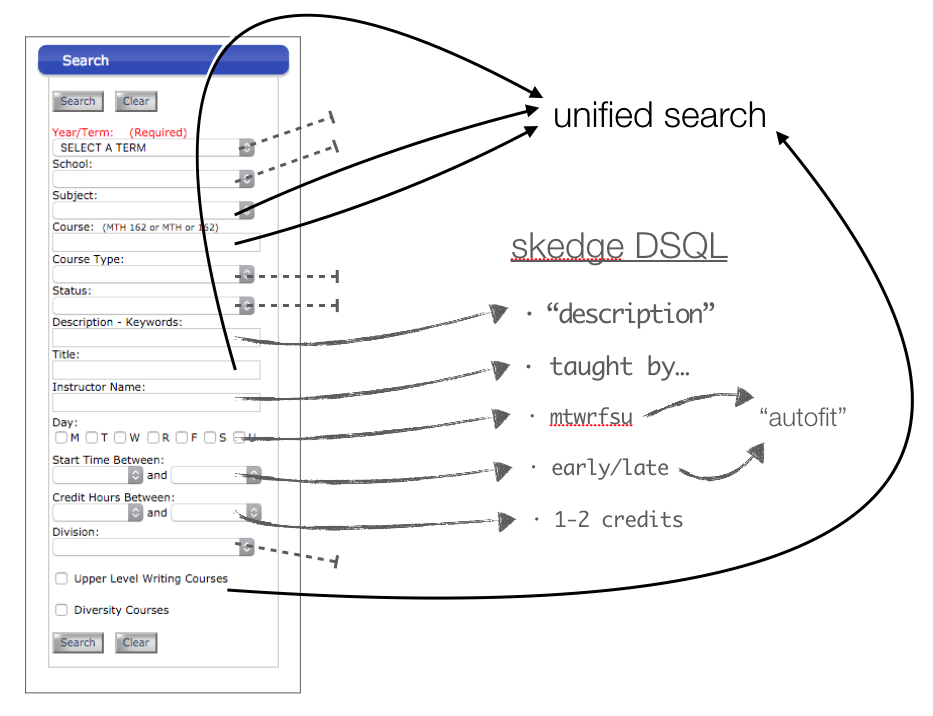
\includegraphics[width=14cm]{images/search-mapping}
  \caption{Mapping from CDCS's form-based search to the Skedge DSQL} \label{fig:search-mapping}
\end{figure}

Figure \ref{fig:search-mapping} is a mapping of each CDCS field to an element of the Skedge DSQL or unified search. Dashed lines that end abruptly are fields that were deemed unnecessary or redundant due to a Skedge-unique feature. To briefly sum up my rationale for each field:

\onehalfspacing

\subsubsection{Removed fields}

\begin{enumerate}

  \item \emph{School} (e.g. ``College of Arts, Sciences, \& Engineering'', ``Eastman School of Music'', etc.) was removed in favor of always searching all schools, as is the default on CDCS. Searching by department codes (which are unique across schools) designates a school regardless.

  \item \emph{Course Type} (e.g. ``Main Course'', ``Lab'', ``Workshop'' etc.) was removed because Skedge already embeds subsections into courses.

  \item \emph{Status} (i.e. ``Open'', ``Closed'', or ``Cancelled'') was removed because it is often useful to see closed courses if there is possibility of the instructor letting in more students, and searching for cancelled courses did not seem useful.

  \item \emph{Division} (i.e. ``Humanities'', ``Social Sciences'', etc.) was removed because it seems too broad to be useful, but it could be added to the Skedge DSQL if there is demand.

\end{enumerate}

\subsubsection{Unified Search (left side)}

The \emph{unified search} components can be entered directly into the single Skedge search field, along with the Skedge DSQL. It includes the CDCS fields:

\begin{enumerate}
  \item \emph{Subject} (department).
  \item \emph{Course} (department code and/or course number, e.g. ``csc 171'').
  \item \emph{Title} (course title).
\end{enumerate}

\subsubsection{Skedge DSQL (right side)}

The \emph{Skedge DSQL} is enterable using special keywords and, optionally, qualifiers for those keywords. It includes the CDCS fields:

\begin{enumerate}
  \item \emph{Year/term}, which is no longer required. It maps to the keywords {\tt \{spring,fall,summer,winter\}} and a four-digit year to specify term and year, and defaults to the current year and term.

  \item \emph{Description}, which is specified by surrounding the query in quotes (e.g. ````buddhism'''').

  \item \emph{Instructor name}, which is specified with the keyword {\tt taught by} and given the instructor name as a qualifier (e.g. ``taught by Guo'').

  \item \emph{Day}, which can be specified with the keywords {\tt \{m,t,w,r,f,s,u\}} for filtering by specific days of the week (e.g. ``mwf'' for Monday-Wednesday-Friday classes only).

  \item \emph{Start time between} is replaced by the keywords {\tt \{early,late\}} which \emph{sort} (ascending and descending, respectively) the results by start time.

  \item \emph{Credit hours between} is replaced by the keyword {\tt credits}, qualified with a number or range (e.g. ``dan 1-2 credits'' for Dance classes with 1-2 credits).

  \item \emph{Upper level writing} is replaced by the single-letter keyword {\tt w} (e.g. ``his w'' for History upper-level writing courses).
\end{enumerate}

\doublespacing

\noindent As noted in Figure \ref{fig:search-mapping}, many use-cases for the \emph{Day} and \emph{Start time between} fields can be obsoleted with an \emph{autofit} feature that will be described later in the next subsection.

  \subsubsection{Advantages of the DSQL}

    The main advantage of Skedge's search system is in its reduction of 15 fields to a single one. I hypothesize that since the vast majority of searches fit the department code / course number pattern (this hypothesis later supported in Chapter 4), the time required to force the user to select a term and then find the correct box to enter this query is wasted.

    In addition, once learned and remembered, using a natural language based query language can be faster and more intuitive than clicking on form fields. And more importantly, the Skedge DSQL is more easily extendable as new search features are invented. For CDCS, the more form fields that are added to the sidebar, the less usable its user interface becomes. For Skedge, while it may take longer for users to learn a bigger DSQL, there is no issue with crowding user interface real estate.
  
  \subsubsection{Disadvantages of the DSQL}

    One disadvantage of Skedge's DSQL is the possible grammatical ambiguity of some queries. For instance, the query ``Fall of the Roman Empire'' could be searching for courses with that as the title, or searching for courses in the \emph{fall term} with the title ``of the Roman Empire''. Unless multiple queries are run and more complex natural language processing is done, the system would have a hard time disambiguating between the two. This could also be solved with a ``did you mean?'' feature, which disambiguates a query into every possible DSQL breakup.
    
    Another notable disadvantage of the DSQL is having to know it, and it having a possibly steep learning curve for some users. However, the argument will be made in Chapter 4 that simply by using the site over time, users will self-learn the Skedge DSQL. One of the ways this is possible is thanks to Skedge's search system being \emph{multi-purposed}. Hyperlinks around the site---instructor names (which link to ``{\tt taught by <name>}''), course references, or schedule course blocks for example---all direct the user to an ordinary search results page with the search field populated, signalling to the user that such a search is possible.


\subsection{Course selection criteria}

I have identified \emph{three} use-cases for course searching (the existence of and distinction between these cases will be demonstrated with collected usage data in Chapter 4). The three cases are \textbf{requirements}, \textbf{electives}, and \textbf{peer recommendations}. The Skedge DSL and other application features offer substantial improvements over CDCS for each of these cases. 

  \subsubsection{Requirements}

  These are courses that are required for a student to complete their degree, and are typically searched for directly. The functionality required here is simple and is mostly satisfied by CDCS, but Skedge offers the following improvements to the process:

  \begin{enumerate}
    \item \emph{Crosslisted courses:} For students with more than one major and/or minor, searching for courses that are crosslisted between departments can be valuable in reducing their requirement load. This search filter is unsupported by CDCS, and is supported by Skedge using the operator ``{\tt x}'' (e.g. ``{\tt csc x ece}'' for courses listed under both Computer Science and Electrical \& Computer Engineering departments).

    \item \emph{Clusters:} Skedge already stores a users' previously taken courses, so it can intelligently suggest either already-completed clusters or courses that would complete clusters that are missing one or two courses. For students with many degree requirements already, this could greatly reduce time spent navigating the University's Cluster Search Engine (for which I also have a long list of grievances, but that lies outside the scope of this paper.)\footnote{This feature is under development and is not currently live. It was, incidentally, requested by a Skedge user.}

    \item \emph{CRN:} Surprisingly, search by Course Reference Number is unsupported by CDCS. It is supported by Skedge by just searching the 5-digit number.
  \end{enumerate}

  \subsubsection{Electives}

  Elective courses can either be courses that are required for a major or minor, but are chosen by the student, or they can be courses of particular interest to students who have the flexibility to take them. For this use-case, Skedge offers search, filter, and sorting features that substantially aid users in browsing through courses and discovering ones they might want to take. Note that none of the following features are supported by CDCS.

  \begin{enumerate}

    \item The Skedge DSQL includes the ``new'' keyword, which qualifies an accompanying search by only displaying the courses that were not offered the previous year for that term. For instance, searching ``new csc'' today (Fall 2016) would show Fall Computer Science courses that have been added to the catalog or changed since Fall 2015.
    \item The Skedge DSQL could include an ``autofit'' keyword, which would take into account the user's current schedule, and only show sections that would not conflict with any already scheduled times.\footnote{This feature is under development and is not currently live.}
    \item The Skedge DSQL includes the ``random'' keyword, which displays a single random course matching the accompanying query. For instance, ``random csc'' would show a random course in Computer Science for the current term. Used in conjunction with ``autofit'', it can a powerful way to find interesting new classes that are available for users to try.
    \item The Skedge DSQL includes sorting by class size---useful for students trying to find smaller, discussion based classes---or by class starting time---for students with preferences of morning or afternoon/evening classes.
    \item Instructor names appearing in courses automatically link to searches for more courses taught by that instructor, which is easier than having to use the CDCS ``instructor'' field to make a separate search.

  \end{enumerate}

  \subsubsection{Peer Recommendations}

  CDCS currently has no support at all for peer course recommendation, a highly undervalued resource for course finding. Skedge implements peer recomendations through Skedge Social, a system detailed in the next section.
  